%
% File naaclhlt2018.tex
%
%% Based on the style files for NAACL-HLT 2018, which were
%% Based on the style files for ACL-2015, with some improvements
%%  taken from the NAACL-2016 style
%% Based on the style files for ACL-2014, which were, in turn,
%% based on ACL-2013, ACL-2012, ACL-2011, ACL-2010, ACL-IJCNLP-2009,
%% EACL-2009, IJCNLP-2008...
%% Based on the style files for EACL 2006 by 
%%e.agirre@ehu.es or Sergi.Balari@uab.es
%% and that of ACL 08 by Joakim Nivre and Noah Smith

\documentclass[11pt,a4paper]{article}
\usepackage[hyperref]{naaclhlt2018}
\usepackage{times}
\usepackage{latexsym}

\usepackage{url}

%%%LK: I added the lines below:
\usepackage{rotating}
\usepackage{tikz}
\usetikzlibrary{shapes,arrows}
\usepackage{graphicx}
\usepackage{tikz-dependency}
\usepackage{natbib}
\usepackage{amsmath}
\DeclareMathOperator*{\argmax}{arg\,max}
\DeclareMathOperator*{\argmin}{arg\,min}
\usepackage{tikz-qtree}
\usepackage{multirow}
\usepackage{rotating}
\usepackage{booktabs}
%% MD: some versions of latex need this package to be loaded last
%\usepackage{gb4e}
%%%LK: I added the lines above

%\aclfinalcopy % Uncomment this line for the final submission
%\def\aclpaperid{***} %  Enter the acl Paper ID here

%\setlength\titlebox{5cm}
% You can expand the titlebox if you need extra space
% to show all the authors. Please do not make the titlebox
% smaller than 5cm (the original size); we will check this
% in the camera-ready version and ask you to change it back.

\newcommand{\param}[1]{\texttt{#1}}
\newcommand{\md}[1]{\marginpar{\scriptsize MD: #1}}
\newcommand{\lk}[1]{\marginpar{\scriptsize LK: #1}}
% for removing all marginpars ==> good for final submission! %%nice trick!
%%\renewcommand{\marginpar}[1]{}

\newcommand\BibTeX{B{\sc ib}\TeX}
\title{Annotating Picture Description Task Responses for Content Analysis}

\author{Levi King \\
  Indiana University \\
  {\tt leviking@indiana.edu} \\\And
  Markus Dickinson \\
  Indiana University \\
  {\tt md7@indiana.edu} \\}

\date{}

\begin{document}
\maketitle
\begin{abstract}
My abstract ...

\end{abstract}


\section{Introduction}

% motivations
% \begin{itemize}
% \item why are we doing what we're doing?
% \item why should someone care?
% \end{itemize}

% Who should care:
% \begin{itemize}
% \item Everyone working with learner data needs to account for its variability
% \item Anyone who wants to deal with acceptability needs to have a definition of what acceptability means
% \end{itemize}

% Our work:
% \begin{itemize}
% \item provides dimensions of acceptability
% \item variability is based on form-meaning matches, and to understand it means knowing what the person intended the meaning to be.  To study variability, we need to control for meaning.  (trick: we don't really know intention, but we do know what the acceptable meaning is for a picture.)
% \end{itemize}

%%Chapter 3, �Special Problems of Language Learners,� outlines the special properties of learner errors, which are often very different from the errors that native speakers make because of the influence of the learner�s native language. We go into some detail presenting three common errors in learner language: those involving prepositions, articles, and collocations.

The (written) data of second language learners poses many challenges, whether it is being analyzed for grammatical errors \citep{leacock:ea:14}, for linguistic patterns \citep{kyle2015automatically}, for content analysis \citep{weigle2013english}, or for interactions with intelligent computer-assisted language learning (ICALL) systems \citep{amaral:meurers:user:07}. One of the core issues in doing anything with learner data is the inherent amount of variability in how linguistic forms are used to convey meaning \citep{Meurers.Dickinson-17}. It may indeed seem like learners can use an infinite variety of forms to express a particular meaning. 
%
But the question of how large the problem of variability is for computational processing has rarely been investigated. More specifically, within the space of possible language productions, there is the further question of determining which are acceptable ones for a given setting.
%Taking this as an overarching question, 

Our overarching goal is to investigate these questions of variability and acceptability, both for non-native speakers (NNSs) and native speakers (NSs), given that all users of a language can be creative in their language usage.
%
To that end---and taking \textit{variability} to concern different mappings between linguistic form and its meaning---in this paper we control for meaning by collecting a dataset of picture description task (PDT) responses from a number of NSs and NNSs, and we annotate a handful of dimensions, thereby capturing the multifaceted ways in which responses can vary and can be acceptable.  Outlining the decisions to be made highlights questions that need to be addressed by anyone working with learner language properties like variability, acceptability and native-likeness.
\md{I note that you don't use an Oxford comma, so I'm trying not to :)}

% \begin{itemize}
% \item Background, purpose of the corpus; (variability within NS and NNS groups; and these groups vary from each other?)
% \end{itemize}

Given the form-meaning aspect of variability, we are interested in how variable linguistic behavior is \emph{for the same content}, both within and among NSs and NNSs.  There is a long-standing notion that systems processing learner data would be wise to constrain the data in some way \citep{heift:schulze:07, somasundaran:chodorow:14, somasundaran:ea:15}, \lk{Is this kind of what you had in mind?}\md{In part.  I added another ref.} but we do not know how much constraint is truly needed, and at what the cost is in terms of losing particular learner behavior for a constraint, without knowing more about the ways in which variation happens \citep[see in particular][]{bailey:meurers:08}.  Even today, the enterprises of ICALL and grammatical error correction (GEC), under their different conditions, would benefit by knowing more about the sources of difficulty in processing the range of learner data they do.

In annotating different dimensions of PDT responses, not only are we able to see how variable they are, but we are able to get a better handle on what could make a particular response ``better'' or ``worse'' for different kinds of purposes.  For example, knowing that a person has gotten the main content of a picture correct, while adding information not present in the picture, may be treated differently than one who has made no such inferences but seems to be addressing a question about a different person in the picture (see section~\ref{sec:scheme}).  The goals of this work are thus distinct from GEC \citep{leacock:ea:14} and from more linguistically driven work such as parsing \citep[e.g.,][]{cahill-et-al:14, ragheb:dickinson:14a}, in that the acceptability of a response is taken as a function of several interacting features, most of which relate the text to the known semantic content.  At the same time, providing the dimensions of acceptability and elucidating how they can be applied provides insight for any enterprise that desires to connect learner text with semantic content, in addition to unpacking the nature of variation more generally.

% \begin{itemize}
% % \item Motivate this for people who don't do this kind of work; measuring 'goodness' of responses; decomposing them into features; (this is not like grammatical error detection or parsing work); Getting a handle on variability, especially under different circumstances; is a response 'native-like'? in what ways (by which features?); breaking variability down into our features;
% \item Anyone working on the automatic processing of learner data can benefit from better understanding the range of variability, and anyone who wants to speak of learner data as diverging from native data needs to qualify the exact nature of that divergence.
% \item Our work:
%   \begin{itemize}
%   \item provides dimensions of acceptability
%   \item variability is based on form-meaning matches, and to understand it means knowing what the person intended the meaning to be.  To study variability, we need to control for meaning.  (trick: we don't really know intention, but we do know what the acceptable meaning is for a picture.)
%   \end{itemize}
% \item Cite previous work:
%   \begin{itemize}
%   \item ours \citep{king:dickinson:13} 
%   \item and others' \citep{somasundaran:ea:15}
%   \end{itemize}
% \end{itemize}

Taking a cue from \citet{king:dickinson:13}, in section~\ref{sec:pdt} we outline the picture description task (PDT) we use, designing items that elicit specific types of linguistic behavior.  Section~\ref{sec:annotation} outlines the annotation, specifically tackling the five-dimensional scheme in section~\ref{sec:scheme} and providing inter-anntotator agreement results in section~\ref{sec:agreement}.  While agreement seems reliable, highlighting areas of disagreement showcases difficult areas for establishing a link between form and meaning \citep[cf., e.g.,][]{Meurers.Dickinson-17}.

\section{Picture Description Task}
\label{sec:pdt}

The PDT is built around 30 cartoon-like vector graphics. The images were modified to remove any non-essential detail or background; some examples are in Table~\ref{tab:test-sample-items}. To factor out the influence of previous linguistic context, images are devoid of any text or symbols, with the exceptions of two images containing numerals, two with music notes, and one with a question mark. Each image depicts an ongoing or imminent action, performed by a person or an animal. The images are divided evenly into intransitive, transitive and ditransitive actions. 

\marginpar{MD: Why do we distinguish targeted from untargeted items?}
Two main versions of the PDT were used. In each version, the first half contains ``targeted'' items, where questions take the form of \textit{What is $<$subject$>$ doing?}, with the subject provided (e.g., \textit{the boy}, \textit{the bird}). The second half contains ``untargeted'' items, where each question asks \textit{What is happening?}. A roughly equal number of targeted and untargeted responses were collected for each item.

Each half (targeted and untargeted) is introduced with instructions, including an example item and responses. The instructions ask participants to focus on the main event depicted in the image and to respond with one complete sentence. The PDT was presented as an online survey and all participants typed their own responses. Participants were instructed not to use any reference materials, but they were permitted to use browser-based spell checking.

In previous similar work \citep{king:dickinson:13,king:dickinson:16}, NSs were found to produce less variation than NNSs. Many NSs provided the same or very similar response with the most canonical way of expressing the main action. One purpose of the current corpus is to be able to assess NNS response content by comparing it against the NS responses; thus, NSs were asked to provide two non-identical responses, in the hopes that this would result in more examples of native-like responses for the variability of NNS responses to compare against.

\subsection{Data Collection}
PDT versions;

NS vs NNS (1 vs 2 responses); 

NNSs demographics (ELIP recruited); 

NSs demographics and sources (known persons vs crowdsourced);

Response counts (types, tokens)

\section{Annotation}
\label{sec:annotation}
The data were annotated with the aim of providing information that would be useful for the automatic assessment of NNS responses via comparison with the NS responses.  A five-dimension annotation, discussed in section~\ref{sec:scheme}, was developed to capture different facets of assessment; insights gained from the annotation, and in particular an interannotator agreement study, are covered in section~\ref{sec:agreement}.

\subsection{Scheme}
\label{sec:scheme}
The annotation scheme was developed through an iterative process of annotation, discussion and revision, with input from two annotators and multiple language professionals. The initial scheme was planned as a three-point scale, ranging from \textit{accurate and native-like} (2) to \textit{accurate but not native-like} (1) to \textit{not accurate} (0). This proved problematic, however, as \textit{accuracy} and \textit{native-likeness} could not be adequately defined and applied to the data.
%\marginpar{MD: A quick example of inadequacy would be nice here.}
For example, in the middle picture of Table~\ref{tab:test-sample-items}, it is not clear how accurate or native-like \textit{She is happy with the dog} is.  Grammatically, it is native-like, but it does not seem like an appropriate answer to the question, \textit{What is the woman doing?}

To address the specifics of appropriate answers, five binary features were eventually settled on, with each feature having some relation to the original concepts of accuracy and native-likeness. A set of annotation guidelines were produced with definitions, rules and examples for each feature. The features and brief descriptions are listed here and discussed further in the following sections:

\begin{enumerate}
\item \textbf{Core Event}: Does the response capture the core event depicted in the image? Core events are not pre-defined but should be fairly obvious given the nature of the images. The response should link an appropriate subject to the event.  In the top picture of Table~\ref{tab:test-sample-items}, \textit{The woman is running} clearly captures the core event, while \textit{She is wearing a red shirt} is irrelevant to the event happening.
\item \textbf{Answerhood}: Does the response make a clear attempt to answer the question? This generally requires a progressive verb. For targeted items, the subject of the question must be used as the subject of the response; appropriate pronouns are also acceptable.  For example, in Table~\ref{tab:test-sample-items}, \textit{XXX} is answering a question other than \textit{What is the woman doing?}
\marginpar{MD: Add faulty example, as this feature is non-obvious}
\item \textbf{Grammaticality}: Is the response free from errors of spelling and grammar?  While the focus of GEC work, in our data set, this is a relatively straightforward feature to annotate (see section~\ref{sec:agreement}).
\item \textbf{Interpretability}: Does the response evoke a clear mental image? Any required verb arguments must be present and unambiguous.  For example, in Table~\ref{tab:test-sample-items}, \textit{XXX} is too vague to generate a clear mental image.
\marginpar{MD: Add faulty example, as this feature is non-obvious}
\item \textbf{Verifiability}: Does the response contain only information that is true and verifiable based on the image? Inferences should not be speculations and are allowed only when necessary and highly probable, as when describing a familial relationship between persons depicted in the image.  For example, in Table~\ref{tab:test-sample-items}, \textit{XXX} conveys information that is irrelevant to the core event but is nonetheless recoverable from the photo (annotation=1), while \textit{YYY} has information that cannot be inferred from the picture.
\marginpar{MD: Add examples}
\end{enumerate}

\subsection{Agreement}
\label{sec:agreement}
Two annotators participated in the annotation. Both are native speakers of English, and each has several years of language teaching experience with both children and adult learners. Annotator 1 (A1) annotated the complete corpus. Annotator 2 (A2) annotated only the development set and the test set, data subsets described next.

Three items were used as a development set for creating and revising the annotation scheme. These items were also used as examples in the guidelines. They represent one intransitive, one transitive and one ditransitive item. Both annotators annotated the full development set multiple times throughout the process, discussing and adjudicating disagreeing annotations before moving on to the test set, which was completed with consultation between the annotators.

The test set parallels the development set and consists of one intransitive, one transitive and one ditransitive item; it is shown in Table~\ref{tab:test-sample-items}. Agreement and Cohen's kappa scores are given in Table~\ref{tab:agreement}, broken down by different criteria.  We will now walk through these results.

\subsubsection{Intransitives, transitives \& ditransitives} Comparisons of the intransitive, transitive and ditransitive items reveal an association between lower item complexity and higher agreement. The highest raw agreement and Cohen's kappa scores are found with the intransitive item, and the lowest are found with the ditransitive item. \marginpar{LK: A type-token ratio table would be helpful here.}

This is as expected, as ditransitive sentences are longer with more verb arguments, meaning there are a greater number of opportunities for responses to vary, and thus more opportunities for annotators to disagree on a given response. This trend also matches annotator feedback; both ranked the ditransitive item as the most difficult to annotate (for all features) and the intransitive as the easiest.

\subsubsection{Targeted \& untargeted} When the annotations are grouped into targeted and untargeted sets, the raw agreement scores are comparable: 94.9\% for targeted and 95.2\% for untargeted items. However, despite a greater degree of response variation, the untargeted group has a higher kappa score: 87.2\% compared to 82.3\%. \marginpar{are kappa scores percentages?} This may appear counterintuitive, but can most likely be attributed to the stricter annotation rules for targeted items. For example, \textit{answerhood} does not allow targeted responses to modify the subject provided in the question in any way. The untargeted questions elicit a greater degree of variation, but the annotation scheme accommodates this. 

When asked to compare the annotation of targeted and untargeted responses, A2 noted that targeted responses require more concentration and closer consultation of the guidelines. Both A1 and A2 describe the annotation of untargeted items as less restrictive.

\subsubsection{Features} Grouped by feature, the annotations all show raw agreement scores above 91\% and Cohen's kappa scores above 74\%. For the future use of this corpus in content assessment, these kappa scores are comfortably above the 67\% commonly suggested as a baseline for meaningful, reliable agreement [CITATION].

\paragraph{Core event} This feature is the most relevant of the five for content assessment. All five features are skewed toward \textit{yes} annotations, but with an average \textit{yes} rate of 72.5\%, core event is the least skewed; i.e., more responses receive a \textit{no} annotation for core event than for any other feature.

Core event has the second lowest inter-annotator agreement kappa score, at 80.8\%. This is somewhat lower than expected, as it is lower than the pre-adjudication development set score (88.9\%). This appears to be largely attributable to the difficulty of the ditransitive item, which was challenging for both participants and annotators. The development set item depicts a man delivering a package to a woman, and many participants were familiar with the appropriate vocabulary and constructions. The test set item shows a man giving directions to a woman, and this resulted in a greater degree of variation, as many NNSs did not describe this in a canonical way. \marginpar{Need to back this up with some numbers!} Rather than constructions like \textit{asking X for directions} or \textit{giving directions to X}, many NNSs describe the item with phrases like \textit{pointing}, \textit{guiding}, \textit{helping a lost person} or \textit{reading a map}, and most disagreeing core event annotations involve such responses, with A2 more likely than A1 to accept these less specific descriptions.

To a lesser extent, the transitive item, which shows a woman hugging a dog, resulted in disagreements where A2 accepts the word \textit{pet} as the object, but A1 rejects such responses as too vague. Despite the acceptable scores for core event agreement, the fact that many disagreements hinge on particular word choice or annotators having minor differences in interpretation of the event suggest that greater agreement could be easily achieved by providing annotators with suggestions about the acceptable content for each response. 

\paragraph{Answerhood} This feature was added largely as a way to identify responses that do not follow the instructions. Such responses tend to fall into three categories: responses that simply do not directly answer the given question; responses that are gibberish or very low-effort and entered only so the participant can proceed to the next item; and ``troll'' responses that attempt to be funny or obscene at the cost of attempting a direct answer.

The majority of participants do attempt to follow the instructions and answer the question, however, and it is unsurprising that this feature skews strongly toward \textit{yes} annotations and results in the highest raw agreement (98.2\%) and kappa (93.6\%) scores among the five features.

Of 23 disagreements, seven stem from an annotator failing to enforce the requirement that a targeted response subject be either an appropriate pronoun or the exact subject given in the question, without adjectives, relative clauses or other modifiers. (This rule separates the task of verifying information from the task of identifying an attempt to answer the question.) Given the question \textit{What is \textbf{the woman} doing?}, for example, the responses \textit{The \textbf{lady} is running} and \textit{The woman \textbf{who in pink} is running} were incorrectly accepted by one annotator. Another 10 disagreements involve responses lacking a progressive verb, which is generally required here as an indication that the response refers to the specific action in the image and does not merely describe a state or a general truth. This suggests that a annotator fatigue accounts for more the majority of answerhood disagreements.

\paragraph{Grammaticality} This is the most heavily skewed feature, with an average \textit{yes} rate of 83.3\%.

Grammaticality has a raw agreement score of 93.0\% and a kappa of 82.7\%. Among 52 disagreements, annotators agreed in discussion that 19 involve an avoidable annotator error. These are primarily responses with typos, misspellings, subject-verb disagreement and bare nouns, which are all rejected by the annotation rules. Such cases are likely attributable to annotator fatigue.

The remainder reflect an unavoidable level of disagreement. Many of these stem from differing interpretations of bare nouns as either errors or as acceptable mass nouns, as in \textit{The man is giving \textbf{direction} to the tourist}. In several disagreements, annotators could not agree on the acceptability of prepositions, as in \textit{The girl is asking for help \textbf{to} the man} and \textit{The girl is hugging \textbf{with} her cat}.


\paragraph{Interpretability} The average \textit{yes} rate for interpretability is 80.2\%; only core event is less skewed.

The raw agreement score is 91.9\% and the kappa is 74.4\%, and these are the lowest agreement scores among the five features. This was anticipated, because interpretability is the most difficult feature to define and leaves much room for annotators' personal judgments. Annotators must decide whether a given response evokes a clear mental image, regardless of how well that mental image matches the PDT image. The guidelines place some restrictions on this mental image. If one were to illustrate it, the result would be a complete, representational, canonical image. It would not be necessary to guess at major elements, like subjects or objects. Any verb arguments in the response would be identifiable in the image -- not obscured or out of the frame. Vague language should be avoided, but human gender does not need to be specified, especially when a non-gendered word like \textit{doctor} or \textit{teacher} is natural. A response like \textit{A woman is receiving a package} fails these criteria, because the person or entity delivering the package is not specified, and an illustrator would need to either guess or compose the image with the deliverer out of the frame. \textit{A man is delivering a package}, would be accepted. An illustrator could simply show a delivery person carrying a package; an indirect object would not be necessary.

Among the 105 annotator disagreements, fatigue accounts for roughly 30; this is difficult to determine precisely because annotators expressed difficulty in identifying a single root cause for many disagreements. Those that are clearly attributable to annotator error tend to involve responses with some internal inconsistency, like subject verb disagreement, making the number of subjects or objects uninterpretable. Among the true disagreements, the level of specificity is often the point of contention. For example, A1 accepted several transitive item responses with the verb \textit{love}, as in \textit{The woman loves her dog.} In discussion, A2 explained that these are too vague to illustrate as an action; A1 disagreed, and this seems to indicate differing judgments regarding the use of \textit{love} as a dynamic verb.

\paragraph{Verifiability} The average \textit{yes} rate for verifiability is 83.1\%, making it the third most skewed feature.

The raw agreement score is 96.8\%, and the kappa score is 88.4\%. By both measures, this is the second highest agreement score, after answerhood. Of 42 disagreements for verifiability, annotators agree that at least eight are avoidable. Of these, five involve the incorrect use of plurals, as in \textit{A man is pointing the way for the women}, when the image shows only one woman. Two other errors stem from inaccuracy, with respondents referring to a dog in the illustration as a cat. One error involves the uninterpretable misspelling of a crucial object, which renders the response unverifiable.

The remaining disagreements are attributable to different opinions about inferences, and in general, A2 is more strict with verifiability.  For the ditransitive item, for example, both annotators accept responses that refer to the woman as a \textit{hiker}, but only A1 accepts responses where both the man and woman are referred to as hikers. For the intransitive item depicting a woman running, A1 accepts multiple responses that refer to this as \textit{a race}, as well as responses that infer the runner's motivation (fitness, leisure, etc.).

\begin{table}[t!]
\begin{center}
\begin{tabular}{|l|c|c|}
\hline
\multicolumn{3}{|c|}{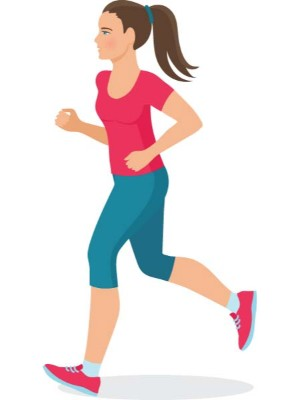
\includegraphics[width=0.35\columnwidth]{figures/I30.jpg}} \\
\hline
%\multicolumn{3}{|l|}{What is the woman doing? [Intransitive]} \\
What is the woman doing? [Intrans.] & A1 & A2 \\
\hline
The woman is running. & 1 & 1 \\
\hline
She is wearing a red shirt. & 0 & 0 \\
\hline
Trying to run from her bad decisions. & 1 & 0 \\
\hline
\hline
\multicolumn{3}{|c|}{
\includegraphics[width=0.35\columnwidth]{figures/I29.jpg}} \\
\hline
What is the woman doing? [Trans.] & A1 & A2 \\
\hline
She's holding a puppy \& looks happy. & 1 & 1 \\
\hline
She is happy with the dog. & 0 & 0 \\
\hline
The lady loves her dog. & 1 & 0 \\
\hline
\hline
\multicolumn{3}{|c|}{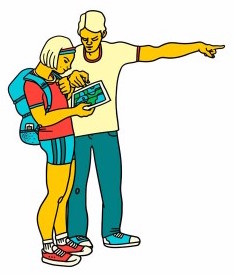
\includegraphics[width=0.5\columnwidth]{figures/I28.jpg}} \\
\hline
What is the man doing? [Ditrans.] & A1 & A2 \\
\hline
giving directions to a woman. & 1 & 1 \\
\hline
The man is reading a map. & 0 & 0 \\
\hline
The man is is telling her where to go. & 1 & 0 \\
\hline
\end{tabular}
\caption{\label{tab:test-sample-items} Test sample items and example responses with Core Event annotations from Annotators 1 and 2.}
\end{center}
\end{table}

\begin{table*}[t!]
\begin{center}
\begin{tabular}{|l|l|l|l|l|l|l|l|}
\hline
Set	& Total	& A1Yes & A2Yes & AvgYes & Chance & Agree & Kappa \\
\hline
\hline
intrans & 2155 & 0.863 & 0.855 & 0.859 & 0.758 & 0.978 & 0.910 \\
\hline
trans & 2155 & 0.780 & 0.774 & 0.777 & 0.653 & 0.949 & 0.880 \\
\hline
ditrans & 2155 & 0.812 & 0.786 & 0.799 & 0.678 & 0.924 & 0.764 \\ 
\hline
\hline
Target & 3390 & 0.829 & 0.818 & 0.824 & 0.709 & 0.949 & 0.823 \\
\hline
Untarg & 3075 & 0.806 & 0.790 & 0.798 & 0.678 & 0.952 & 0.872 \\
\hline
\hline
Core & 1293 & 0.733 & 0.717 & 0.725 & 0.601 & 0.923 & 0.808 \\
\hline
Answer & 1293 & 0.834 & 0.831 & 0.833 & 0.721 & 0.982 & 0.936 \\
\hline
Gramm & 1293 & 0.861 & 0.872 & 0.866 & 0.768 & 0.960 & 0.827 \\
\hline
Interp & 1293 & 0.818 & 0.787 & 0.802 & 0.682 & 0.919 & 0.744 \\
\hline
Verif & 1293 & 0.845 & 0.817 & 0.831 & 0.719 & 0.968 & 0.884 \\
\hline
\end{tabular}
\caption{\label{tab:agreement} Agreement scores for different groupings of the test set, showing total annotations, \textit{yes} annotations for Annotator 1 and 2, average \textit{yes} annotations, total expected chance agreement (\textit{yes} + \textit{no}), actual raw agreement and Cohen's kappa.}
\end{center}
\end{table*}

\smallskip

Relevant tables:\\
Types, Tokens, TypeTokenRatio \\
(for targeted vs. untargeted) \\

\section{Discussion}

\subsection{Annotator feedback}
Annotators' impressions of the task; 

what is difficult? what is easy?

\subsection{Agreement \& Disagreement Trends}
(Do trends align with annotator feedback?)

What kinds of items \& responses were challenging?

Are the trends for individual features? Recurring disagreements?


\subsection{Limitations}
what we'd do differently:

which images are problematic and why (symbols, ambiguity); 

Which features are problematic; useful/not useful;

\subsection{Potential Uses}
Use of corpus in the next phase of my work;

Suggestions of other projects and research questions for this corpus.

\section*{Acknowledgments}

(Advisors, annotators)
\bibliographystyle{acl_natbib.bst}
\bibliography{levi-bib.bib}

%The acknowledgments should go immediately before the references.  Do
%not number the acknowledgments section. Do not include this section
%when submitting your paper for review. \\
%
%\noindent {\bf Preparing References:} \\
%
%Include your own bib file like this:
%\verb|\bibliographystyle{acl_natbib}|
%\verb|\bibliography{naaclhlt2018}|
%
%Where \verb|naaclhlt2018| corresponds to a naaclhlt2018.bib file.
%\bibliography{naaclhlt2018}
%\bibliographystyle{acl_natbib}
%
%\appendix
%
%\section{Supplemental Material}
%\label{sec:supplemental}
%Submissions may include resources (software and/or data) used in in the work and described in the paper. Papers that are submitted with accompanying software and/or data may receive additional credit toward the overall evaluation score, and the potential impact of the software and data will be taken into account when making the acceptance/rejection decisions. Any accompanying software and/or data should include licenses and documentation of research review as appropriate.
%
%
%NAACL-HLT 2018 also encourages the submission of supplementary material to report preprocessing decisions, model parameters, and other details necessary for the replication of the experiments reported in the paper. Seemingly small preprocessing decisions can sometimes make a large difference in performance, so it is crucial to record such decisions to precisely characterize state-of-the-art methods. 
%
%Nonetheless, supplementary material should be supplementary (rather
%than central) to the paper. {\bf Submissions that misuse the supplementary 
%material may be rejected without review.}
%Essentially, supplementary material may include explanations or details
%of proofs or derivations that do not fit into the paper, lists of
%features or feature templates, sample inputs and outputs for a system,
%pseudo-code or source code, and data. (Source code and data should
%be separate uploads, rather than part of the paper).
%
%The paper should not rely on the supplementary material: while the paper
%may refer to and cite the supplementary material and the supplementary material will be available to the
%reviewers, they will not be asked to review the
%supplementary material.
%
%Appendices ({\em i.e.} supplementary material in the form of proofs, tables,
%or pseudo-code) should be {\bf uploaded as supplementary material} when submitting the paper for review.
%Upon acceptance, the appendices come after the references, as shown here. Use
%\verb|\appendix| before any appendix section to switch the section
%numbering over to letters.
%
%\section{Multiple Appendices}
%\dots can be gotten by using more than one section. We hope you won't
%need that.

\end{document}